\documentclass{data/hbue}

%在这里添加需要使用的宏包
\usepackage{hyphenat}
\usepackage{amsmath}
\usepackage{textcomp}
\usepackage{xcolor}
\usepackage{minted}

\begin{document}

\newminted{cpp}{linenos, numbersep=5pt, frame=lines, framesep=2mm}
\newminted{python}{linenos, numbersep=5pt, frame=lines, framesep=2mm}
\newminted{javascript}{linenos, numbersep=5pt, frame=lines, framesep=2mm}

%读取封面信息
%用来生成论文封面和开题报告封面信息

%论文{题目}
\hbuetitle{局域网大文件并发传输设计与实现} 

%学生{姓名}
\hbueauthor{夏彬}

%指导老师{姓名}{职称}
\hbuementor{宋莺}{讲师} 

%{所属院校}{专业}{年级}{班级}{学号}
\hbueinfo{信息管理学院}{计算机科学与技术}{S1021}{2010}{1032149}

%{开题报告时间}
\hbuereporttime{2011年1月1日}


%生成封面
{%使用{}防止cover内修改的一些参数影响正文
\thispagestyle{empty}
\newcommand{\ulbox}[1]{\ul{\makebox[6cm]{#1}}}
\renewcommand{\baselinestretch}{2.5}

\fbox{\wuhao\heiti\sinfog 届普通本科毕业论文\-(设计)}
\hfill
{\wuhao\heiti 存档编号:\ul{\makebox[1.4cm]{}}}

\sanhao

\begin{center}
	
\includegraphics[scale=1.1]{data/images/badge.png}

	{\chuhao\textbf{毕业论文\-(设计)}}
	\vspace{2.5em}

	题目: {\ul{\makebox[13cm]{\bfseries{\erhao\stitle}}}} \\[2cm]
	\begin{tabular}{lc} 
		专\hspace{2em}业:& \ulbox{\kaiti\sinfop}  \\ 
		院\hspace{2em}系:& \ulbox{\kaiti\sinfos} \\
		年\hspace{2em}级:& \ulbox{\kaiti\sinfog 级} \\
		学\hspace{2em}号:& \ulbox{\kaiti\sinfon} \\
		姓\hspace{2em}名:& \ulbox{\kaiti\sauthor} \\
		指导老师:& \ulbox{\kaiti\smentorn} \\
		职\hspace{2em}称:& \ulbox{\kaiti\smentort} \\ 
	\end{tabular}

	\vfill
	{\heiti 湖北经济学院教务处\hspace{1em}制} 
\end{center}
}


\frontmatter\pagenumbering{Roman} %目录本身要求使用大写罗马编页号

%生成目录
\tableofcontents

\mainmatter

%以下为具体章节文件.
\chapter*{摘要}

本文通过设计并实现了一款局域网内的并发传输工具,
可以有效解决同一文件多次传输时的重复发送问题.
以此工具的实现过程介绍了linux下软件开发的常用方式,
利用C++11的新特性使代码更加简洁, 使用python等脚本语言
的优势进行代码生成和测试. 

\noindent\textbf{关键字:} WEB UDP Linux C++11 git Python CMake

\chapter{绪论}
\section{前言}
本次设计题目来源于在校期间曾多次遇到教师上课时需要发送一些文件给学生安装
以便更好的进行教学安排,但在文件较大时局域网即使处在满负荷之下也无法满足
人数众多的学生同时下载。因此萌生使用UDP的广播特性来进行文件传输这一想法。
考虑到操作系统的多样化以及自己一直是在linux环境下成长的,因此跨平台是
这款软件的一个必备要求。

本次设计和实现均在linux下使用开源工具完成意义在于,
在桌面计算机上主流的三种操作系统有linux、Mac和Windows。
国内Windows在过去占据着主导位置,随着苹果这几年的崛起国内IT公司已经开
始注重其他系统平台用户。现在国内很多软件都已经拥有Mac版本,少部分软件
拥有linux版本。而且手机、平板这些便携式电脑已经越来越流行,软件平台早
已不再局限在Windows上。也不会局限在某一特定事物之上。
跨平台不仅仅意味着能在多个系统上运行,同时促使软件开发人员在开发软件时
尽量不用操作系统特性而是使用更具抽象性的工具如C++的boost库。这样能更好
的进行抽象设计,而不用过早陷入细节问题。

本次设计主要是基于以太网的特殊性,在物理层每张网卡都会接收到局域网内所有
的数据\cite{TCP/IP},UDP本身是不适合进行大文件传输的特别是在互联网上,但合理使用广播或多播
这种利用以太网本身的传输机制进行合理的利用带宽,就可以让这种并发传输
的情况下非常明显的``突破''网络物理限制。
可以节约宝贵的时间,特别是在课堂上。

\section{本文研究的内容和结构}
第2章介绍了开发环境以及开发中使用到的一些技术和工具,包括操作系统平台,
文本编辑器,编译器,项目管理工具和版本控制等。

第3到5章讨论了软件的核心设计包括核心数据结构,发送接收过程。

第6章介绍了用户界面的选择以及介绍了为更好的使用WebPage作为界面而
另行设计的一款HTTP服务器AppWebServer。

第7章介绍了界面的js/html代码部分主要谈论了在使用WebPage时遇到的
一些问题和选择。

第8章简单的介绍了本次测试使用的一些方式。

\chapter{开发环境}
本章介绍了系统中使用到的一些开发工具和系统环境。
首先介绍了使用的操作系统同时稍微比较了一下linux和windows的各自优缺点。
然后列举了使用的开发工具并没有使用IDE进行开发,IDE是一个很大的进步但
亦有其缺点,并且命令行下的构建工具也是在发展。
这里介绍的工具和windows下的开发方式有较大区别本文只简单介绍使用的工
具不过多的阐明原因,
对于长期使用IDE的朋友可以选择看一下云风的一篇连载文章``IDE不是程序员的
唯一选择'',这里并非争论谁更高效,只是希望每个人都能有机会进行选择。

\section{系统环境}
开发环境是archlinux系统(其他linux系统同样适用),
Arch Linux的官方介绍很简短:
\begin{quote}
``A lightweight and flexible Linux\textregistered \ distribution that tries to
Keep It Simple.``
\end{quote}
将近5年的日常使用感受是它很符合官方介绍所说的KISS原则,保持linux的简单和灵活。
它不像其他发行版有固定的版本号,archlinux使用pacman和aur进行滚动升级,类似
gentoo的管理方式,但常用软件官方有提供二进制包。可以让你在第一时间使用到最新的
软件版本。

windows和linux的一个很大区别,windows很多工具都比linux下要更加方便
(但一般都是收费软件且价格不菲)。windows下由于主要是靠商业程序来丰富应用因此它上
面的程序一般会比较好用但于其他软件的交互上基本已经让用户错误的认为程序间不需要
什么交流。
linux下则不同大部分软件虽然完成的功能很单一接口也不是很友好,但十分容易和其他
工具结合起来用,用户可以任意选择各种工具组合起来,可以在遇到好用的工具
后将其集成到自己的工作环境中。linux下大部分软件的接口都会有其常用的约定,
比如-s以便代表大小(可能是指示显示文件大小或者是按照文件大小排序);
-h一般是指human表示使用较友好的输出格式或者是help的意思。
有时候对于第一次使用的工具会在没有看帮助信息的情况下自然的使用到正确的
指令(当然仅仅是非常通用的)。

在linux你可以把绝大部分重复的工作自动化,比如在编写这款软件的时候需要在虚拟机
里面测试windows下的运行情况,需要来回的拷贝编译好的文件到虚拟机去执行。在厌烦
最初的几次拷贝后便编写了几行脚本来完成这个工作,现在只需要进入WIN32目录下make
一下就可以自动编译最新的版本且自动将文件拷贝到windows中。在切换进win系统后就可
以直接运行了(当然也比较容易做到make之后让win下最新的版本自动运行)。

linux也有其不方便的地方比如桌面软件很多情况下需要考虑win下用户的使用造成调试
繁琐;它的图形接口在稳定的前提下没有Windows友好; 
国内大部分商业公司的软件均不支持linux;
完成同一件事情会给你过多的选择(虽然这一点也可以算作优点),造成刚刚进入某个
领域时对于选择什么工具或技术十分困难。

这里选择linux仅仅是因为长期使用的原因,我个人是很少学习linux系统本身的API。因此
不会使用linux本身的特性,尽量保证程序能做到平台无关。

\section{开发工具}
\subsection{文本编辑器}
在windows下学习编程的同学可能很少有文本编辑器的概念,我在接触linux之前也只了解
记事本这个简陋的软件;Word这种处理文档的工具;VB6.0、Dreamware等集成开发环境。

现在编程语言如此之多,对于一个稍有好奇心的人来说都仅仅使用一种语言是残酷的。
因此如果说现今什么编辑工具最可能支持所有的语言那肯定是非vim和emacs莫属了。
这里选择使用vim作为代码编辑工具原因很简单它是一个优秀的文本编辑器而,并且也只
熟悉这一个文本编辑器。

在软件编写和论文撰写阶段至需要编辑python代码、C++代码(且需要支持刚刚发布的11标
准的部分新语法和工具)、html代码、Javascript代码、CSS代码、latex代码以及CMake的
配置文件。
这仅仅只是在完成这个简单的毕业论文需要应付的语言。而在日常学习生活中需要遇到的
文件类型更是各种各样,仅仅我个人平常需要编辑的文件种类都可以继续列出许多。

如果每种文件都使用特意为其编写的工具来编辑那么在计算机这个日新月异的发展速度下
你在学习某种技术的时候就需要花费一些不必要的额外时间。而使用vim这类工具你
需要的仅仅是在遇到一种新语言或文件的时候在网络上花上十多分钟就能获得不错
的效果。
除了少数通用约定(如ctrl+v,ctrl+z,alt+<F4>之类)你在一个工具上积累的知识
很可能在下一个工具上就不再适用了。 而使用文本编辑器你可以解决任何纯文本格式
的编写问题,你所积累的会越来越多你的效率也会随之提高。
因为其设计理念它不会随着时代的变迁而变的不再适用(至少vim的前身vi的年龄比我
要大)。

vim和emacs在网上已经有很多中文资料我在此就不在这里介绍了。

如果没有vim这样的文本编辑器则在本次论文过程中就很难处理众多的文件格式。

\subsection{编译器}
C++的编译器种类并不多成熟的只有GCC,VC,Intel C++以及新秀clang(Apple主导
研发的基于LLVM的编译器)。
其他如TrubC++、Borland C++由于失去支持我觉得即使作为教学也不该使用。
Intel C++口碑不错但是商业程序,VC2010有express版但只能在win下使用。
clang++对c++11的支持不够多,因此这里选择gcc4.6.2作为主要的工具。
win下的编译工具使用mingw。 win下面使用在发布的时候选用vc++进行编译也许是
更好的选择。

在交叉编译上这里介绍一个叫做mingw cross的项目。这个项目主要是帮助用户在
linux下建立一整套完整的交叉编译工具(仅仅针对win32)和常用的库。通过脚本进行
构造最简单的情况下可以仅仅下载完脚本文件一个make命令后自动下载源代码自动
编译大部分软件库(比如qt,gtk等),如果手动编译的话会有很多问题而这个项目
通过测试特定版本对有问题的地方给出workaround的path从而大大简化了交叉编译。

\subsection{构建工具}
这里使用CMake进行构建管理。CMake通过读取配置文件CMakeLists。txt来生成makefile
文件。可以方便的进行工程管理。
较老的资料都是介绍GNU的Autotools系列工具,只是这套工具还是稍嫌麻烦,当然
其历史悠久稳定可靠。
但如果不是为了开发完全符合gnu规则的软件则使用CMake是十分好的选择。
另外CMake可以生成其他IDE需要的工程文件比如VS。

如果使用Java语言则Ant是最好的选择了。
还有两款使用python写的C/C++构建工具SCons和Waf也有一定名气。

本次使用CMake来管理项目使编译过程变得十分轻松,不论是交叉编译windows下的可执行
文件还是linux下的可执行文件都只需使用同一份CMakelists。txt进行管理一个make命令
就行了。

\subsection{版本管理}
这里仅仅讨论开源的版本管理软件。
Git是较新的版本管理软件05年才刚开发出来,而我也只是这几年才了解。
Git作者对其名称来源是这样解释的:
\begin{quote}
``I'm an egotistical bastard, and I name all my projects
after. First Linux, now git.''
\end{quote}
从First Linux就知道这句话是Linus Torvalds说的了,他也是git的最初作者。

因为早期使用的商业软件BitKeeper合作到期Linux社区急需一款优秀的版本管
理软件来管理日益庞大的Kernel,所以创造了Git。

这之前最流行的开源CVS是软件要属SVN了,著名的sourceforge就是使用svn
进行代码托管的,Google Code也是, 国内的Sina App Engine也是。
我最初使用的CVS也是svn,但svn需要开启一个服务进程稍显麻烦。
CVS虽然是Concurrent  Versions System的缩写但它同时也是一款历史悠久
的版本管理软件的名称。

使用版本控制几乎已经成为软件开发中必须的一个环节了,特别是git的出现
是部署版本管理的成本几乎为零,你所需要做的仅仅是在命令行下敲入git init
就行了。
在编写代码时候就多次利用git的分支功能进行一些想法上的实践,如果没有
版本控制就必须出现一个想法的时候把源代码复制保存一份以免破坏原有代码。

\subsection{文档工具}
这里使用的latex是指编写本论文的工具,而非软件文档。
如果所写程序属于供他人使用的代码库则可以用doxygen自动生成
文档。
本论文很少涉及到数学公式而且没有现成的模板文件因此使用latex并非是一个
很好的选择,但考虑到linux下使用libreoffice(基本可以认为是OpenOffice)
会在一些细节地方与MS Word不兼容且自身对word类工具使用经验较少。
因此选择latex这类用户不需要关注版式但却能很自动排版的工具。
其中中文宏包使用xeCJK。
利用latex使本次论文的编写不需要关注论文版式上的问题\footnote{当然在没有
模板的情况下还是需要花一定时间去调整版式,因此特意将完成的latex模板放在
github.com上以便以后的同学使用latex编写本校论文不需要关注论文格式。}。

\chapter{核心数据结构}
由于UDP缺乏可靠性\cite{UDP}可能出现丢包、出错、复制等现象,
并且缺乏拥塞控制机制(congestion control)。
对于丢包、出错等现象对于需要绝对安全的文件传输来说是绝对不能允许的,
对于大文件的传输如果没有拥塞控制则可能出现大量丢包(通过之前
做本地回环实验丢包率可达到30\%,实际局域网不会这么高),或者由于传输
间隔过长导致效率急剧下降。

因此必须设计特定结构来克服这些困难。


\section{散列函数}
散列函数(Hash Function)
Hash Function可以从任何一种数据中创建较小的数字``指纹'',它可以把
很大的数据量压缩成较小的固定位数的数字\cite{hash}.

这里Hash代表系统的一个数据结构struct Hash;
通过使用Hash结构来对某一事物进行唯一标示。
准确的唯一标示应该使用UUID,但UUID只是产生一个唯一标示符但不能和对
应的事物产生关联。

在表示文件时使用Hash进行唯一标示以免文件名相同但内容不同的文件出现。
在传输数据的时候使用Hash对传输的数据块进行完整性验证以保证最终收到
的文件不会有任何字节偏差\footnote{传输二进制文件必须保证没有任何字节出错。}。

最出名的Hash算法要属MD5,MD5常用来对用户密码进行加密(稍微安全一些
的做法是加上salt)。
另外还有SHA-0,SHA-1,SHA-256,SHA-512更安全的算法也较为出名。

考虑到计算量以及允许出现碰撞情况的出现,这里没有选用上面这些较好的
Hash算法,而是使用计算量较低的MD4,没有使用MD2的原因是MD2使用16位
整型进行操作在32位或者64位CPU上不一定会带来速度的提升。

源码中仅仅使用typedef将一个string作为Hash类型
typedef std::string Hash;
具体计算hash是通过
Hash hash\_data(const char* data, size\_t size);
函数调用\mbox{crypto++}库的md4函数进行计算。


\section{文件的抽象表示}
在有操作系统和文件系统的支持下我们可以方便的使用文件路径进行文件定位
以及操作。
而进行网络传输时则需要把文件的一些必备信息告诉对方
这里涉及到文件大小,文件有多少块,一次发送整个文件是不理智的UDP协议也
因为length字段仅仅16位\cite{UDP}所以一次最多只能传送大约64Kb的数据,一块数据
有多大,文件名和真实路径,文件类型等问题。

这里先将系统使用的数据结构给出
\begin{cppcode}
struct FInfo {
	enum Type : uint8_t {
		NormalFile, Directory, RootFile, RootDir 
	} file_type;
	enum Status { 
		Local, Downloading,Remote 
	} status;
	Hash parent_hash;
	Hash hash;
	uint32_t chunknum;
	uint16_t lastchunksize;
	std::string path;
}
\end{cppcode}
enum Type 使用了c++11的新特性\cite{cpp11}用来指定enum底层的数据
类型\footnote{默认为int。},因为\mbox{C/C++}的基本类型并非固定大小因
此在进行网络传输时必须使用定长类型或者
对变长类型\footnote{path字段就是变长的。}进行特殊处理。
uintXX\_t在c++11中是作为标准类型出现的(定义在cstdint中)。
enum Status由于不需要在网络中进行传输仅仅是在本地进行状态变迁使用的,所以
无须指定底层类型。

FInfo可以通过info\_to\_net和info\_from\_net这一组函数在网络上进行传输。
chunknum表示文件有多少块数据;
普通文件块的长度是一个在config.hpp中定义的
固定值\footnote{当前通过考虑选择60000。}
lastchunksize表示最后一块数据的
长度\footnote{文件长度不会总能被60000整除。}。
通过这2个变量和一个常量就可以计算出某个文件的大小以及文件块数。

path在不同情况下意义稍有不同,在文件正在传输时path指向了操作系统中对应
文件的真实路径\footnote{上传者和下载者一般是不同路径的。}。
刚通过网络接收后但还没
开始进行下载时path仅仅保存了文件的名称以便用户大概知道文件的内容。
由于path字段是变长大小因此在进行传输时需要进行特定处理,这里使用的方式
是用一个uint8\_t代表path长度,在进行传输和接收时自动处理。因此path的长度
固定在1~256之间,超过这个长度系统会自动截断但会优先保留后缀名以便用户
有机会通过后缀名初步判断此文件是否需要。

hash字段是通过对整个文件进行hashing得到的16位定长数据,可以很好的用来区别
不同文件。

status字段是用来表示当前文件状态的,刚从网络接收到的FInfo都是Remote状态,
开始下载后转换为Downloading状态,下载完成后成为Local状态。
如果FInfo是本机制造的则为Local状态。

以上几个字段就可以很好的处理普通文件传输了,但如果需要传输目录则需要进一般
处理,这里增加了file\_type和parent\_hash两个字段来完成。
共有4种文件类型普通文件(NormalFile),目录(Directory),根文件(RootFile),
根目录(RootDir),其中RootFile和RootDir不需要parent\_hash这个字段(因此在进行
实际传输时会根据文件类型来判断是否发送或接收parent\_hash)。
为了较容易理解这里举出一个例子:
假如使用data作为路径来建立FInfo则会产生以下7个FInfo出来。
\newpage
\begin{verbatim}
|-- data  				//RootFile
|   |-- cover.tex   	//NormalFile  -> data.hash
|   |-- hbue.cls		//NormalFile  -> data.hash
|   |-- images			//Directory   -> data.hash
|   |   |-- badge2.png 	//NormalFile  -> images.hash
|   |   `-- badge.png 	//NormalFile  -> images.hash
|   `-- report_imp.tex	//NormalFile  -> data.hash	
其中->指向的是parent_hash
\end{verbatim}
这里仅仅是在进行普通文件传输的原基础之上改造了一个传输目录的方式,但
并不建议使用目录传输方式,特别是这里设计的方式有大量冗余信息。因为目录
传输的缺点在于文件数量非常多的时候速度会急剧下降建议使用tar,rar,7z等能进行
打包\footnote{在unix下很常见的一种方式并非是压缩,处理速度很快。}后传输。
这种目录传输方式有一个好处是用户可以有选择的仅仅下载目录中部分文件,
并且FInfo不需要一次性传输,可以在打开RootDir的时候仅仅获取下一级的目录,这样就
类似于AJAX技术,在不影响用户体验的时候减少不必要的传输。


\section{文件完整性和分块}
如果传输的是视频、音频等文件丟几个字节没有很大关系,这也是使用UDP的主要原因,
但很可惜本系统无法利用UDP的这些优点,必须保证文件的完整。
UDP会出现丢包、重复、乱序等问题。
但都可以通过分块传输来解决。
数据结构如下:
\begin{cppcode}
struct Chunk {
	Hash file_hash;
	Hash chunk_hash;
	uint32_t index;
	uint16_t size;
	const char* data;
}
\end{cppcode}
Chunk表示一个文件块;
file\_hash表示此文件块所属文件;
chunk\_hash是此文件块所携带数据的hash值;
index表示此文件块在整个文件中的序号;
size表示所携带数据长度;
data在发送时携带size长的真实数据,在发送前仅仅指向数据地址。

这里同样使用的都是定长类型,以便在不同操作系统下可以顺利完成通讯。
其中chunk\_hash在发送前进行hashing,接收者在接收到一个文件块后如果通过
计算发送所携带数据和chunk\_hash不符则直接丢弃。

顺便说明这里能够表达的最大文件大小并非$2^{16}*2^{32}$一是因为实际大小
和文件系统有关,二是在下面要介绍的数据结构Bill中也会有限制。

\section{文件块的请求}
因为是分块发送的,所以请求者无法直接发送一条类似GIVE\_ME\_FILE\_XXX这样
的指令到网络然后就等着接收文件\footnote{UDP的丢包、重复、乱序等造成。}。
因此需要使用特定的结构来进行特定文件块的请求。
这里使用Bill结构,示意代码如下:
\begin{cppcode}
struct Bill {
  Hash hash;
  uint16_t region;
  BlockType bits;
};
\end{cppcode}
hash表示请求的文件hash;
region表示当前区域;
bits表示此区域内的请求信息。

BlockType在config.hpp中定义为typedef uint32\_t BlockType是一个32位无符号类型。
bits中的某一位若为1表示需要此块文件若为0表示不需要。这里因为需要进行网络传输
因此使用了uint32\_t结构,但实际操作时是转换为std::bitset<\mbox{BLOCK\_LEN}>
类型来方便位操作。
由于这个结构只提供通讯的辅助信息但又是需要大量发送的,所以需要尽量高效的利用
空间。在bits和region的类型选取上进行了一定考虑。
BlockType不能太小否则会蜕化为一次请求一块的效果了。但也不能太大否则就成了一次
这里选取region为16位可以表达65536个区域,
每一个区域可以携带32块信息,每一个最多携带60000B数据(BLOCK\_SIZE)因此可以
表达出$32 * 2^{16} * 60000 \approx 117。1875GB$ 大小的文件。
整个Bill占用空间sizeof(Bill) = 16 + 16 + 32 刚好等于64,在32位操作系统和64位
操作系统下都已经是对齐的结构。

\section{丢包率}
本系统中由于Bill的数据量较小在局域网中不会造成太大影响。
因此这里只考虑大量发送Chunk时的情况。
TCP使用的拥塞控制算法\cite{TCP}有``慢启动''(slow start),
``拥塞避免''(congestion avoidance),``快速重传''(fast retransmit)
和``快速恢复''(fast recovery)具体见TCP/IP详解\cite{TCP/IP}。
TCP的这些算法很多是面向环境恶劣的Internet网络,而这篇论文所讨论的系统
只需要处理合理控制好发送间隔就能很好的处理问题。

处理方法仅仅是根据一个interval(int类型)的值来在发送chunk的时候进行一定
时间的延迟,这个值的计算是通过整个网络的丢包率进行动态计算的大小在0$\sim$32
之间,
\[\textrm{丢包率}:\omega = \frac{interval}{32。0} * 100\%\]
\[\textrm{间隔时间}:i = \omega * 40ms\]
这里选用40ms作为最大值是通过粗略估计算的出:\\
设M为网卡带最大带宽,单位byte/;,\\
则在满带宽情况下计算出每1byte需要使用的时间$s = \frac{1000}{M}$,单位ms;\\
然后计算出发送一块文件块的时间 $t = s * 60000$;
采用典型的网卡设备100Mbps和1Gbps分别计算得出4。6ms和0。46ms的结果,
再用同样的方式计算硬盘读取的速度,
假设硬盘读取速度30Mb/s,算出读取一块数据需要2ms。
即使再加上CPU处理时间一块数据的处理时间不会超过10ms。
实际代码中接收端是通过多线程写入数据只要收到数据后可以忽略写入时间。
因此40ms在局域网已经是非常保守的值了,初始状态interval的值是0。
具体如何计算interval需要设计到其他结构因此在下一章
的``速度统计与丢包率''中进行介绍。

\chapter{文件发送与接收}
本章介绍先后尝试的三种传输模型:``一问一答''、`并发处理''、``多此迭代''。
最终通过分析综合考虑选择使用``多次迭代''。

这一章由于涉及到的概念并非十分具体因此为了更好的表述做以下约定:
\begin{itemize}
	\item S为发送者。
	\item $R_x$为接收者,如$R_1,R_2$等。
	\item 涉及的文件拥有N块数据\footnote{FInfo.chunknum字段的值。}。
	\item 当前发送的文件块\footnote{即之前介绍的Chunk结构。}为$C_x (0<x<N)$。
	\item 文件块请求以$B_x$\footnote{与之前介绍的Bill有关。}为一组,
		一组包含0~32块请求$0 < x < N/32$。
	\item 最大文件区域的值 $n = N/32$
\end{itemize}
所有文件传输模型均只考虑一对多的方式即一个发送者多个接收者。

\section{一问一答}
采用请求发送模式,R发送需要的文件块到网络中,S收到后发送文件块到网络。
但由于是一对多的发送方式,一份文件可能有多个接收者,导致S重复发送文件块。

例如,一个节点$R_1$开始请求数据后,文件传输途中另外一节点$R_2$发送请求
通讯过程如下:
\begin{enumerate}
	\item $R_1$ 发送$B_1,B_2,\ldots,B_n$ 到网络中;
	\item S收到$B_1\sim B_n$ 后开始发送
		$CB_1,CB_2,\ldots,CB_i (i < n)$;
	\item 在S 未发送完毕时,$R_2$ 开始请求下载,发送
		$B_1,B_2,\ldots,B_n$ 到网络中;
	\item S在发送完 $CB_n$ 后继续发送$CB_1,\ldots,B_i$,
		此时$R_1,R_2$都已经拥有完整的文件拷贝;
	\item S继续发送$CB_{i+1},\ldots,CB_n$到网络中,此时所发数据会
		无故占用网络带宽;
\end{enumerate}

\section{多次迭代}
因此不能使用这种简单的一问一答的方式发送文件块,必须设计一种``智能''的发送方式。

把种方式称做``多次迭代''是因为S只处理比PCR值大的文件块请求,
小于这个值的请求则直接忽略直到没有文件块可传则结束本轮传输。

对于发送者S制定如下规则:
\begin{itemize}
	\item
		维护一个当前文件发送状态STATE 取值范围: BEGIN、SENDING、END
		STATE默认状态为END; \\
		在END状态下$R_x$收到SB命令S转换为BEGIN状态;\\
		在BEGIN状态下收到$B_x$转换为SENDING状态; \\
		在SENDING状态下发送$B_n$之后转换为END状态;
	\item 维护一个指向当前发送文件区域的指针PCR(Point to Current Region),取值范
		围:$0\leq PCR\leq N/32$;\\
		PCR的值仅在SENDING状态下有效; \\
		PCR的值根据收到的最大$B_x$设置,如先后收到
		$B_1,B_2,B_3,B_8,B_4$则PCR的状态先后为1,2,3,8,8;
	\item 在收到$B_x$后若x<=PCR则忽略此$B_x$请求;
	\item 在END状态下忽略一切$B_x$请求;
	\item 从SENDING转换为END时候发送SE;
\end{itemize}


对于接收者$R_x$制定如下规则:
\begin{itemize}
	\item 请求开始时发送SB指令后发送$B_i\ldots B_j$到网络,
		其中$0 \leq i \le j \leq N/32$;
	\item $B_x$请求顺序必须按照升序排列;
	\item 在收到所缺区域中值最大的区域时结束请求。例如所缺文件区
		域为$B1,B2,B3,B4$,当前已经接收到$CB1,CB2$。如果此时接
		收到$CB_4$则直接结束,虽然$CB_3$暂时未收到;

	\item 在收到SE的时候结束当前请求;
	\item 在结束请求后若文件未下载完成则重新开始请求;
	\item 发送的$B_x$序列必须包含$B_n$若不需要此区域的文件块可发送空的$B_n$;
\end{itemize}

按照设定的规则之后,再来看之前遇到的问题:
\begin{enumerate}
	\item $R_1$ 发送$SB$,$B_1,B_2,\ldots,B_n$到网络中;
	\item $S$在收到$SB$后从END状态转换为BEGIN状态,收到$B_1$后从BEGIN转换为
		SENDING状态,并设置PCR=1,在收到$B_2$后设置PCR=2,\ldots 设置PCR=x;
	\item 在S{\em 未}发送完毕时,$R_2$开始请求下载,发送SB,$B_1,B_2,\ldots,B_n$到网络中;
	\item 由于S在SENDING状态忽略SB命令,收到$B_1$,小于PCR=x忽略,$B_2$,
		小于PCR=x忽略;
	\item S在发送完$CB_n$后PCR=n,因此忽略队列之后的请求,
		此时$R_1$拥有完整拷贝,$R_2$拥有$CB_x$之后的拷贝;
	\item $R_1$收到$CB_n$后完成下载退出通讯;$R_2$则结束当前请求发送SE,
		S收到后状态转化为END;
	\item 由于$R_2$结束请求后检测还有未完成的文件块,因此重新开始建立请求,
		发送SB,$B_1,B_2,\ldots,B_{x-1}$;
	\item 此时网络退化为点对点传送\footnote{如果之前有n个$R_x$则
		根据退出数量y蜕化为1对n-y传输。};
\end{enumerate}

不过发送$B_x$的速度很快,例如一个1G的文件根据系统的设
定ChunkSize=60000b,一个Bill最多可携带32块Chunk,一个
Bill的大小是16+16+32=64b,因此所需数据量是,
$(1G/60000b/32)*64=35,791b$ 只有30多Kb在局域网内相对
于人的操作是瞬间完成的。因此更多的时候是这种情况: S
收到的数据是这样
\begin{align*}
	SB,B_1,B_2,\cdots,B_n\\
	SB,B_1,B_2,\cdots,B_n\\
	SB,B_1,B_2,\cdots,B_n\\
\end{align*}
则S对应的处理序列是:发送$CB_1,\cdots,CB_n$后忽略之后队列中所有的$B_x$和SB
此时大部分$R_x$都已经在收到$CB_n$后完成下载。

但由于丢包的原因可能导致部分$R_x$还有少部分数据块未接收到。
这些$R_x$在收到SE后结束当前请求,并根据下载规则重新请求下载。
之后S收到的数据是这样:
\begin{align*}
	SB,B_{x1},B_{x2},B_{x8},B_n         	(R_1)\\
	SB,B_{x2},B_{x7},B_{x8},B_{x10},B_n 	(R_2)\\
	SB,B_{x3},B_{x4},B_{x6},B_n 			(R_3)\\
	\\
	其中x1 \leq x2 \leq x3 \cdots xn,但x1不一定和x2是相邻关系。
\end{align*}

S会根据之前的规则处理
$SB,B_{x1},B_{x2},B_{x8},B_{x10}$
其中后面的SB和$B_{x7},B_{x3},B_{x4},B_{x6}$等都被忽略。
$R_1$在收到$B_{x8}$后完成下载;
$R_2$在收到SE后发送SB,$B_{x7},B_{x10},B_n$到网络;
$R_3$在收到SE后发送SB,$B_{x3},B_{x4},B_{x6},B_n$到网络;\\
此时S收到以下序列:
\begin{align*}
	SB,B_{x7},B_{x10},B_n,SB,B_{x3},B_{x4},B_{x6},B_n
\end{align*}
处理完毕后$R_2$收到所有的文件块结束下载,$R_3$依然没收到任何数据,但收到SE后重
新发送SB,$B_{x3},B_{x4},B_{x6},B_n$ 到网络中,此后完成所有发送过程。

以上过程发生概率虽然不算罕见,但发生时所缺少的$B_x$量一般都会很小因此虽然处理过程
复杂但会很快完成。及时在最坏情况下也会至少处理一个$B_x$请求。而局域网内一般只会几十
人下载收敛速度会非常快。
并且其中$R_3$的数据是特意构造导致前几次的迭代过程中没有收到任何有效的文件块,但
如果分析实际情况,$R_3$所缺少的文件块很可能与其他$R_x$大部分相同。原因在于所缺少的
文件块部分是因为丢包造成的。

如果以上过程中发送的$B_n$因为网络原因丢包了,如果是$R_1$的$B_n$丢包了则会加
快处理速度,因为$R_2$的$B_{x10}$可以不用等待下一次迭代就发送完毕。如果是$R_2$或者
$R_3$的$R_n$丢包了则会导致S和R都停止工作。

因此需要保证S在无事可做时尽快进入END以便通知$R_x$此轮请求结束,同时也需要保证
$R_x$有接收到S发送的SE指令。否则可能导致S和R都在等待对方的信息。
为了防止这种情况的发生,S和R都有一个定时器,S在SENDING状态下一定时间内若没有
发送任何$CB_x$则自动进入END状态。R在一定时间内没有收到文件块也会自动结束当前
请求。

对于文件的发送接收有一个重要原则,宁可让一个$R_x$重新发送全部的$B_x$也不能发送
一块无效的文件块,因为一个文件块就有60000B,而且一般一次发送32块,即使按照平均
长度一次无效的文件块发送也会导致960K的浪费。而前面有计算过1G的文件也只有30K
的$B_x$数据。
而造成重复$B_x$的原因是发送$B_x$的数据量小导致发送速度非常快,往往一个$CB_x$
都还没发送完毕所有$R_x$的$B_x$就已经进入到了S的处理队列中,因此S的队列中有非常
多的重复$B_x$,必须使用一个指针来指名当前位置,到达最后位置的时候就
将队列中所有数据全部抛弃(绝大部分都是重复无效的数据)让$R_x$重新发送请求。

\section{并发处理}
之前还尝试过另外一种模式,使用一个map记录当前系统所缺少的文件块(根据$B_x$来维护
这个map),则如果接收到重复的$B_x$后由于已经有记录了就直接抛弃处理。
这种模式可以很好的解决部分问题,但在实现中必须使用多线程,发送线程和
处理$B_x$线程且需要共享这个map结构,较为麻烦。
且同样需要加入超时机制防止R、S停止工作,重新设
计一种方案,重新请求由于丢包导致$R_x$没有接收到的文件块。可以使用超时重传但效率
过低。而上面讨论的方案由于有多个$B_n$的冗余保证了快速重传(只要不是最后一个$B_n$
丢包了则不会影响效率相反由于$B_n$的丢包导致之后的$B_x$可以继续发送(需要大小PCR的
$B_x$); 

两种方案都可以尽量减少错误的重发文件块,前者通过消耗更多的流量来达到重传机
制,后者虽然不消耗多余的流量但需要消耗宝贵的时间。但在局域网中宝贵的资源是带
宽而不是流量,如果使用超时机制来实现重传则其实在浪费时间的同时浪费了大量的带
宽,因此在最初选择后者之后改为选择前者来实现本工具。

\chapter{系统其他部分}
{\em 本章未完成}
\section{速度统计与拥塞控制}
速度统计分为以下三种
\begin{enumerate}
	\item 局域网内全局有效下载速度;
	\item 单一节点有效下载速度;
	\item 单一节点特定文件有效下载速度;
\end{enumerate}

其中后两者可以只需要根据单节点自身统计信息就可计算出来

PB指向当前还未验证的文件块头, PM指向已经

count([PM,PB]) = THRESHOLD/2
一次最多发送 THRESHOLD块请求

<< R1, R2
>> C1
<< A1, R3, R4, %有待考证
>> C2, C3
<< A3, R5, R6,
>> C4, C5,
<< A5, R7, R8,
>> C6, C7,
>> A7, R9, R10,

<< R1, R2
>> C1,
<< A1, R3, R4
>> C2,
<< A2, R5, R6,
>> C3,
<< A3, R7, R8,
>> C4, C5, C6, C7, C8
-------------
<< A4, A5, A6, A7, A8




\section{文件信息管理}
\section{网络驱动}
\section{系统集成}

\chapter{用户界面库}
本章第一节先介绍一些造初期考虑使用的用户界面程序库(GUI);
第二小节阐述了HTML作为本次设计的选择的原因以及使用这种技术会遇到的一些问题以及解
决方案。
第三小节简要的介绍了作为本次设计而附带产生的一款简单的HttpServer。
第四小节根据实际情况介绍了使用脚本语言来帮助我们简化开发。
\section{常见GUI库}
Win平台专属的库微软本身的MFC,Windows Forms\footnote{dotnet中的winform},
Borland的OWL(Object Windows Library);
Mac平台专属的库Cocoa,
Linux平台由于操作系统本身是没有定义\footnote{unix类系统一般使用X11作为GUI。}
GUI的所以一般来说没有专属GUI库。
由于多平台运行是本次设计的一个硬性目标所以以上GUI库无法采用。

能够提供跨平台支持的GUI库也是非常多,但有的GUI库只提供一种
\footnote{一般专门的GUI库都会有多种语言绑定}编程语言如Java的
AWT,SWT,所以这类GUI也不在考虑范围之类。

还有一些出名的的GUI库如QT,GTK虽然比较熟悉但这类GUI由于不仅仅包含了GUI的内容而且
几乎是从底层完全重写导致编译出来的程序过大
\footnote{根据以往经验使用strip,upx后也会达到5M左右,GTK稍小。},
因此考虑到最终程序的尺寸(footprint)问题,犹豫之后还是放弃了这2个选择。

和QT,GTK类似的一款wxWidget在windows上优化之后可以让最终程序保持在2M左右,
也是我最熟悉的GUI库。

以上介绍的一些GUI库除了Window Forms,AWT,SWT因为和自身平台高度集成其外,
其他GUI库都由于GUI本身的复杂性以及历史原因导致有非常多的东西与现今标准中
的内容重复,但又由于向后兼容以及这些内容已经在库中根深蒂固无法去除。

所以在初期还有考虑过FLTK这款简单的仅仅提供界面部分的GUI库。

但犹豫再三后还是决定放弃以上GUI库,主要原因在于
\begin{itemize}
	\item 使用系统平台提供的GUI虽然可以不明显增加最终程序尺寸,
		但却不具备跨平台的特性;
	\item 使用平台无关的GUI一般会导致最终程序尺寸急剧膨胀;
	\item 一些小巧的GUI库虽然不会导致最终程序尺寸过大但此类GUI一般都较为简陋;
\end{itemize}

因此萌生使用HTML作为程序界面的想法,理由如下:
\begin{itemize}
	\item HTML依托用户的游览器本身来渲染界面,
		可以以最小的代价\footnote{程序大小方面。}来完成界面显示。
	\item 使用JS可以方便的处理界面逻辑,使用CSS灵活的定义显示界面。
	\item HTML作为前端界面已经在暗中普及起来,只有稍微注意就可以发现仅仅国内,
		各大软件的最新版本中Web技术都已经在界面显示上占据越来越大的作用。
	\item HTML可以使设计变得更简单,使用WEB技术意味着你在设计程序的时候就已经强
		制设计者是核心逻辑与界面逻辑分开处理。这样可以让强迫设计者时刻提醒自己核
		心逻辑应该提供出来的接口。同时在多人合作的时候可以并行展开工作。界面部分
		与核心部分可以做到没有任何耦合,他们直接的通讯是通过中间一层简单的包装进
		行联系的。
\end{itemize}
因此在选择WEB技术之后,可以满足程序尺寸的要求,并且能提供更加简单且灵活的界面。

\section{选择WEB的问题}

虽然使用WEB技术有非常多诱人的地方,但凡事都不会完美,WEB也有着宁人烦恼的问题。
\begin{itemize}
	\item 由于种种原因在国内至今存在着大量已经被其开发者淘汰的游览器,这些游览器
		导致同一份文件最终显示效果却不同。
	\item 这一点和上面是对立的,就是如果在程序中内嵌自己的渲染部分则可以保证用户
		体验上的统一,但会急剧增加尺寸。
	\item 由于WEB技术和C++或其他语言写的程序是独立的因此需要自己处理他们之间的通
		讯。
	\item 需要依赖服务器来提供内容。
	\item HTML/CSS/JS/IMG这类文件和应用程序单独分离在发行程序的时候会稍显复杂。
\end{itemize}

对于存在的古老游览器我选择的是稍激进的方法--不予理会。虽然第一感觉是不理智,但新
技术是需要时间和人的推进才会普及起来,这也是现在部分非商业网站选择明确放弃这些游
览器的原因。
这是很多新应用新网站都必须进行的一个困难选择。不过好在各大厂商都在积极的推进
HTML5技术而且和C++11类似,在标准还没正式发布前大部分功能已经在实践中运用了。
这一问题的另外一个缓解方案是使用第三方的JS库来处理游览器的差异,这一点将在下一章
中介绍。

内嵌一个游览器来给用户统一的体验是非常好的选择,但由于尺寸原因导致本文设计的这类
程序无法接受。如果是其他程序如自用,定制产品或大规模的程序都可以选择这种方案,
这里一般可以选择WebKit作为内核进行移植或使用第三方库,如果选择使用QT已经原生支持
WebKit了,其他库或语言一般也会有对应binding。

Web页面需要和应用程序进行信息交换,这一点可以通过jsonp等常规方案解决简单解决,如
果在HTML5普及之后也可以使用WebSocket进行更加完善的处理。

最后两点可以通过一种方案一次完美解决就是自己写一个简单的服务器,通过源码级别集成
到应用程序里,Web页面需要的一些文件在调式完成后就编译进这个服务器内部。

这里选择使用自己编写一款HttpServer的原因主要在于没有找到简单的解决处理最后一点的
方案,如果仅仅是内嵌一款普通HTTP服务器有很多优秀的开源项目可供选择如lighthttpd。

\section{AppWebServer的介绍} \label{sec:aws}
AppWebServer是为了完成本次设计特意另行编写的一款专门用来集成到其他程序里的小型
HttpServer,且提供调式和发行两种模式。调式模式下AWS通过读取指定目录下的文件进行
工作,发行模式下AWS则不读取任何外部文件,直接将文件编译到程序内部。

使用方式十分简单,如下代码就建立了一个简单的HTTP Server,可以读取doc\_root(默认)下
的文件进行工作。
\begin{cppcode}
#inlcude <AppWebServer.hpp>
int main()
{
	AWS::Server s;
	s.run();
}
\end{cppcode}
另外也可以通过注册RPC::Service到Server里去,这样游览器使用js发送一个请求到
``/rpc。cgi''上就可以调用Service提供的函数来获得所需功能。js端发送消息的格式会在
下一章中进行介绍。
这里只讨论后端代码。
注册Service也是很简单的,如以下代码注册一个提供文件系统信息的service到
server里去。
\begin{cppcode}
#inlcude <AppWebServer.hpp>
AWS::Service& rpc_filesystem();
int main()
{
	AWS::Server s;
	AWS::RPCServer rpc;
	rpc.install_service(rpc_filesystem());
	s.set_rpc(rpc);
	s.run();
}
\\...
AWS::Service& rpc_filesystem()
{
	static AWS::Service filesystem;
	//service的名称
	filesystem.name = "filesystem";

	//service的方法列表,以下语法使用C++11提供的lambda语法来编写匿名函数
	//使用Uniform initialization语法来初始化service的方法列表。
	//使用auto语法来自动推导函数返回类型。
	filesystem.methods = {
	{
		//函数名称
		"list_file", 
		//具体的函数代码
		[](const AWS::JSON& j){
		AWS::JSON result;
		if (j["path"].isString()) {
			string p(j["path"].asString());
			for (auto& n : list_file(p)) {
				AWS::JSON node;
				node["type"] = n.type;
				node["path"] = n.path;
				node["name"] = n.name;
				result.append(node);
			}
		} 
		return result;
		}
	},
	{
		\\提供的其他函数。
	}
	};
	return filesystem;
}
\end{cppcode}

一个service由service名称和方法列表组成,一般一个service会提供多个函数。
其中list\_file是完成具体工作的函数,这个函数接受一个路径然后返回此路径下所有的文
件信息。AWS::JSON底层使用的是jsoncpp的json::value,JSON参见\cite{json}。
所有service的函数都会返回一个AWS::JSON类型来表达返回结果,
程序核心部分和界面部分就是根据这些service提供的接口来完成设计的,如需要制作一个提
供文件选择的界面模块则可根据这里提供的filesystem service来实现,WebPage通过传递
一个路径(最开始可以是。代表当前目录)给``filesystem''服务的``list\_file''函数就可以
得到这个目录下的文件信息,然后就可以继续根据得到的信息进行下一步请求。

这个模块也是这次设计中实际碰到的问题,由于文件传输肯定涉及到文件目录,但当前游览
器基于安全考虑都是不允许得到文件路径的,通过``<input type=file>''只能得到文件的
名称而无法获得完整路径。这在普通Web应用上是完全可以理解的,而且已经在现今所以较新
版本游览器中执行了。所以必须要自己实现遍历文件系统的功能,最终实现结果比当初遇到
这个问题预想的要容易多的解决。仅使用100来行的C++和100行的JS代码就完成了这个功能。

下一节介绍完成AWS发行模式使用到的技术。

\section{使用脚本语言来生成资源}
linux下曾多次遇到程序里需要嵌入外部文件的问题,
Win下可以方便的通过资源文件来解决,如win下的icon一般都是作为资源文件放到pe格
式文件里的,并且通过一定的hack手段可以实现动态更新exe里的资源文件
\footnote{比如可以实现配置信息保存到exe文件内。}。
Linux下我曾多次寻找对应技术但没有什么收获,因此一般都是遇到的时候用脚本语
言来生成\mbox{C++}代码作为补救。以前几次是使用Perl来编写,不过因为比较简单写的
也比较凌乱代码没有保留,这次又碰到这个问题因此使用Python来写了一个特意完
成AWS发现模式功能的简单脚本来生成``资源文件''。
脚本默认遍历读取doc\_root目录下的文件,并生成content.hpp和content.cpp文件。
content.cpp里包含了资源内容,content.hpp提供\_RC函数的接口,通过使用这个函数其他
代码就可以方便的得到对应文件的字节码。如获得index.htm文件和js/main.js文件就可以
简单的分别调用\_RC(``/index.htm'')和\_RC(``/js/main.js'')带得到,其中\_RC返回的
是一个array<const char*, size\_t>,
array是C++最新标版本\cite{cpp11}提供的标准类型。
第一个字段指向对应文件的字节码,后一个字段表示文件长度。

脚本文件较为简单不到100行,主要是使用struct的unpack函数\cite{python}来进
行解码。代码如下
\begin{pythoncode}
import sys
import os
from struct import unpack

content_hpp =  '\
/*THIS FILE IS AUTO GENERATE BY AppWebServer Resource Builder*/\n\
\n\
#ifndef CONTENT_HPP_\n \
#define CONTENT_HPP_\n\
#include <utility>\n\
#include <string>\n\
std::pair<unsigned char*, size_t> _RC(std::string path);\n\
#endif\n'

content_cpp = '\
/*THIS FILE IS AUTO GENERATE BY AppWebServer Resource Builder*/\n\
\
#include "content.hpp"\n\
#include <string>\n\
using namespace std;\n\
typedef unsigned char uchar;\n\
	std::pair<uchar*,size_t> _RC(std::string path){{\n\
    static uchar* _rc_empty = 0;\n\
    {0}\n\
    return make_pair(_rc_empty, -1);\n\
}}'
content_static = 'static uchar {0}[] = {{\n {1} \n}};\n'
content_return_first = '\
if (path == "{0}") {{\n\
    return make_pair({1}, {2});\n\
}}'

content_return = '\
 else if (path == "{0}") {{\n\
   return make_pair({1}, {2});\n\
}}\n'

contents = ["", ""]

doc_root = "doc_root/"
if len(sys.argv) == 2:
    doc_root = sys.argv[1]

def generate_one(name, path, template=content_return):
    f = open(path, 'r')
    data = f.read()
    f.close()
    if (len(data) == 0):
        print "Waring: {0} is zero length file!".format(path)
        c = template.format(path, "_rc_empty", 0)
        return ["", c]

    content = unpack("{0}c".format(len(data)), data)
    tmp = ""
    counter = 0
    for i in content:
        tmp += "0x{0:x}, ".format(ord(i))
        counter += 1
        if (counter % 10 == 0):
            tmp += "\n\t\t"
    s = content_static.format(name, tmp)
    c = template.format(path[1:], name, len(content))
    return [s, c]


old_path= os.path.abspath('.')
os.chdir(doc_root)

counter = 0;
for root, dirs, files in os.walk("."):
    for file in files:
        if (counter==0):
            c = generate_one("_rc_{0}".format(counter), 
			os.path.join(root, file), content_return_first)
        else:
            c = generate_one("_rc_{0}".format(counter), 
			os.path.join(root, file))
        contents[0] += c[0]
        contents[1] += c[1]
        counter += 1;

os.chdir(old_path)

f = open("content.cpp", "w")
f.write(content_cpp.format(contents[0]+contents[1]));
f.close()

f = open("content.hpp", "w")
f.write(content_hpp)
f.close()
\end{pythoncode}


这里的解决方案是可以算作是一种很早就有的使用用代码生成代码的方式,QT的特定扩展,
Google的Buffer Protocol都算是这类解决方案。可以利用其他简单的工具辅助我们的工作。

AWS通过这个脚本生成的content。hpp和content。cpp文件就能通过条件编译来选择是使用这
里提供的数据还是直接读取文件系统下的目录。
这样设计之后在代码调式的时候可以直接更改WebPage的内容,而在最终发布的时候便可以仅
仅给用户提供一个可执行文件。

\chapter{界面实现}

\chapter{开发中的测试}
\section{BoostPython介绍}
\section{BoostTest和CPPUnit}

\begin{table}
	\center
	\caption{Mac OS X和Windows比较}
	\begin{tabular}[t!]{ccc}
	\hline
	项目 & Windows & Mac \\
	\hline
	版本 & Windows7 & Mac OS x 10.6 \\
	核心 & NT Kernel & XNU \\
	CLI  & CMD.exe & UNIX shell \\
	GUI  &  Windows Explorer & Aqua \\
	\hline
\end{tabular}
\end{table}

\begin{figure}
	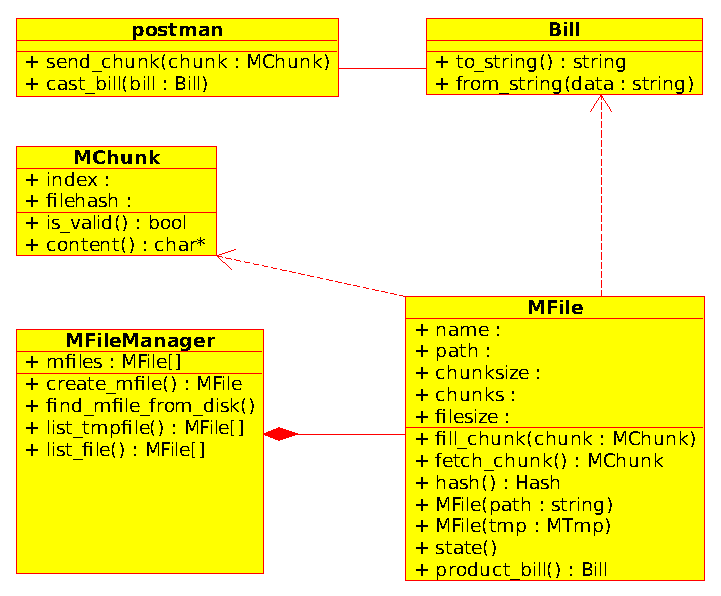
\includegraphics{figure/filemanger.eps}
	\caption{文件管理示意图}
\end{figure}

\chapter*{结束语}
本章未完成
\addcontentsline{toc}{chapter}{结束语}

\begin{table}
	\center
	\caption{Mac OS X和Windows比较,表格测试}
	\begin{tabular}[t!]{ccc}
	\hline
	项目 & Windows & Mac \\
	\hline
	版本 & Windows7 & Mac OS x 10.6 \\
	核心 & NT Kernel & XNU \\
	CLI  & CMD.exe & UNIX shell \\
	GUI  &  Windows Explorer & Aqua \\
	\hline
\end{tabular}
\end{table}

\begin{figure}
	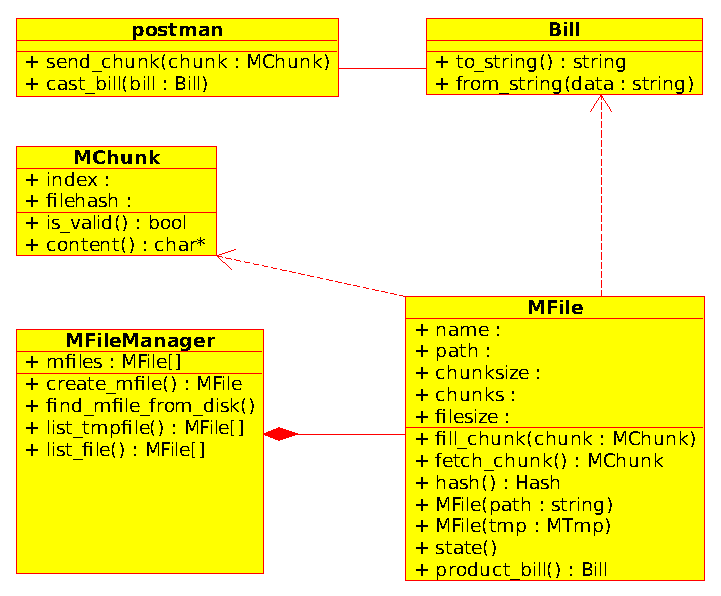
\includegraphics{figure/filemanger.eps}
	\caption{文件管理示意图, 图测试}
\end{figure}


\backmatter

%参考文献
\bibliographystyle{plain}
\addcontentsline{toc}{chapter}{附录及参考文献}
\begin{thebibliography}{99}
	\bibitem{UDP} 
		RFC 768, User Datagram Protocol[S].
	\bibitem{TCP}
		RFC 793, Transmission Control Protocol[S].
	\bibitem{json}
		RFC 4627, The application/json Media Type for JavaScript Object
		Notation (JSON)[S].
	\bibitem{cmake}
		Andrej Cedilnik, HOWTO: Cross-Platform Software Development Using CMake
		,2003-10
	\bibitem{jquery}
		jQuery社区专家, jQuery Cookbook, 东南大学出版社, 2010-10
	\bibitem{cpp11}
		Bjarne Stroustrup, C++11 -the recently approved new ISO C++ standard,\\
		\url{http://www2.research.att.com/~bs/C++0xFAQ.html}
	\bibitem{TCP/IP}
		W.Richard Stevens, TCP/IP 详解 卷1, 机械工业出版社, 2000-4
	\bibitem{thecpp}
		Bjarne Stroustrup, C++程序设计语言, 机械工业出版社, 2002-1
	\bibitem{webdesign}
		Zoe Mickley Gillenwater, 灵活Web设计, 机械工业出版社, 2009
	\bibitem{hash}
		Wikipedia, Hash Function, \url{http://en.wikipedia.org/wiki/Hash\_function}
	\bibitem{vim}
		Steve Oualline, Vi iMproved(VIM), Sams, 2001-4
	\bibitem{css}
		Christopher Schmitt, CSS Cookbook, O'Reilly Media, 2004-8
	\bibitem{less}
		Alexis Sellier, The Dynamic Stylesheet language, \url{http://www.lesscss.net}
	\bibitem{python}
		Mark Lutz, Python编程(第三版英文$\cdot$影印版), 东南大学出版社, 2006
	\bibitem{progit}
		Scott Chacon, Pro Git, Apress, 2009-8
	\bibitem{boost}
		Boost Community, Boost Library Documentation,
		\url{http://www.boost.org/doc/libs}
\end{thebibliography}

\end{document}
